\setlength{\parskip}{\baselineskip} 
\section{PCP}

\begin{frame}
 \frametitle{Table of Contents}
 \vspace{-2em}
\textbf{
\begin{itemize}
 {\color{gray}
     \item {Background}}
     {\color{matbluedark}
         \item PCP}
         \begin{itemize}
         {\color{gray}
             \item Method
             \item Simulations
             \item Application}
         \end{itemize}
          {\color{gray}
         \item \bnmf}
         \begin{itemize}
         {\color{gray}
             \item Method
             \item Simulations
             \item Application}
         \end{itemize}
    {\color{gray}
     \item \bnmf \& Child IQ
     \item Conclusion
     }
 \end{itemize}}
\end{frame}

\frame{
\frametitle{Principal component pursuit}
\begin{itemize}
    \item Robust Principal Component Analysis (PCA)
    \item Data dimensionality reduction method adapted from computer vision
    \item Decomposes design matrix into low rank and sparse
    \begin{itemize}
        \item {\color{matbluedark}Low rank matrix} estimates consistent exposure patterns
        \item {\color{matbluedark}Sparse matrix} identifies unique events \\
        %
        \centering\begin{tcolorbox}[colframe=matbluedark, colback=white, width=6cm, height=1.2cm,halign=center,valign=center]
        \begin{center}
        \only<1>{\vspace{1ex}$$\hspace{-1ex} \min _{L, S} \|L\|_{\star} + \lambda\|S\|_{1} + \frac{\mu}{2}\|L+S-X\|_{F}^{2}$$}
        % %
        \only<2>{\vspace{1ex}$$\hspace{-1ex} \min _{L, S} \mathcolorbox{yellow}{\|L\|_{\star}} + \lambda\|S\|_{1} + \frac{\mu}{2}\|L+S-X\|_{F}^{2}$$}
        % %
        \only<3>{\vspace{1ex}$$\hspace{-1ex} \min _{L, S} \|L\|_{\star} + \mathcolorbox{yellow}{\lambda\|S\|_{1}} + \frac{\mu}{2}\|L+S-X\|_{F}^{2}$$}
        % %
        \only<4>{\vspace{-1.9ex}$$\hspace{-1ex} \min _{L, S} \|L\|_{\star} + \lambda\|S\|_{1} + \mathcolorbox{yellow}{\frac{\mu}{2}\|L+S-X\|_{F}^{2}}$$}
        % %
        \only<5>{\vspace{-2.4ex}$$\hspace{-1ex}\min _{L, S} \|L\|_{\star} + \mathcolorbox{yellow}{\lambda}\|S\|_{1} + \frac{\mathcolorbox{yellow}{\mu}}{2}\|L+S-X\|_{F}^{2}$$}
        \end{center}
        \end{tcolorbox}
    \end{itemize}
       {\item Robust to noisy/corrupt data}
    {\begin{itemize}
        \item Not influenced by outlying values
    \end{itemize}}
\end{itemize}
}

\frame{
\frametitle{PCP image example}

\vspace{-1.75ex}
\begin{center}

\begin{tabular}{ccc}
Original & $\widehat{L_0}$ & $\widehat{S_0}$\\
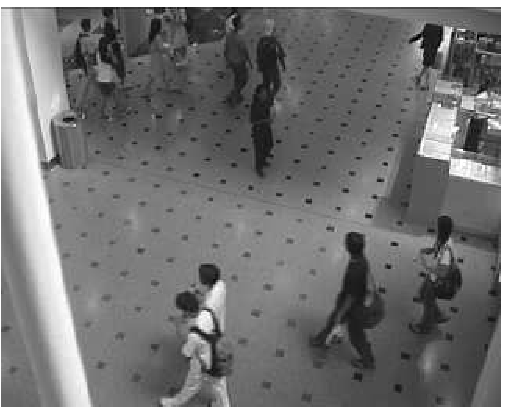
\includegraphics[scale=0.3]{figures/pcp/figure_mall_ori_1.pdf} &
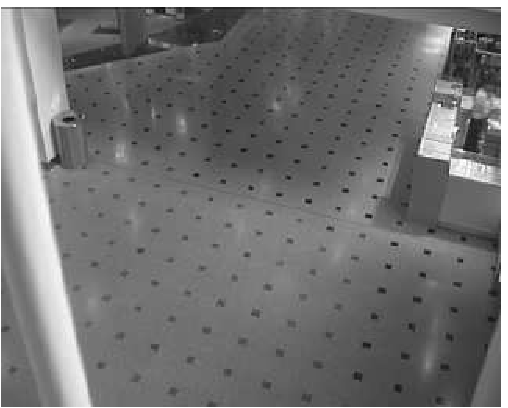
\includegraphics[scale=0.3]{figures/pcp/figure_mall_L_1.pdf} &
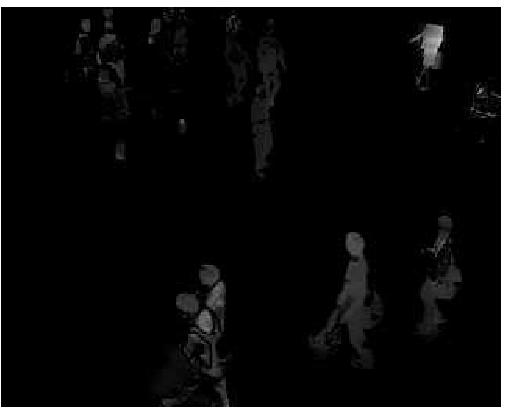
\includegraphics[scale=0.3]{figures/pcp/figure_mall_S_1.pdf} \\

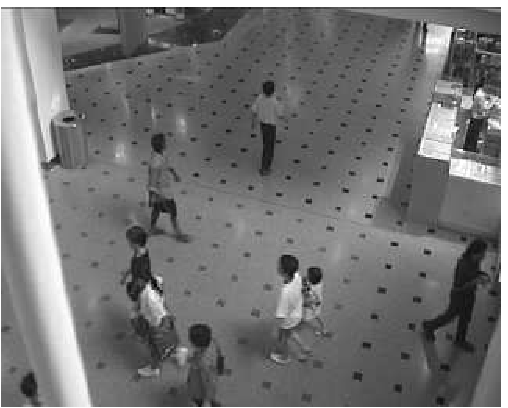
\includegraphics[scale=0.3]{figures/pcp/figure_mall_ori_2.pdf} &
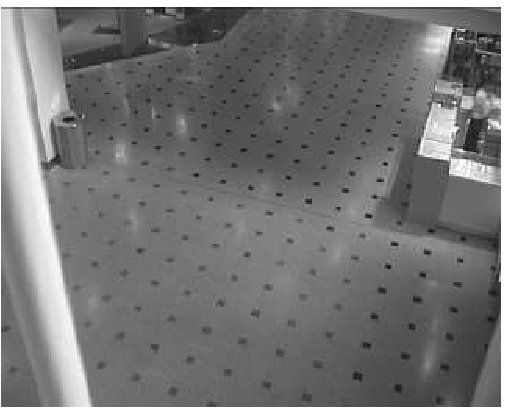
\includegraphics[scale=0.3]{figures/pcp/figure_mall_L_2.pdf} &
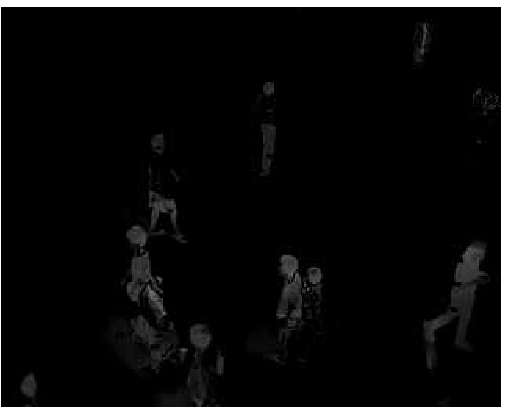
\includegraphics[scale=0.3]{figures/pcp/figure_mall_S_2.pdf} \\

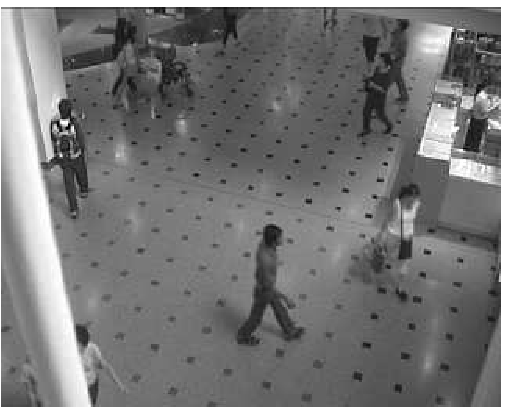
\includegraphics[scale=0.3]{figures/pcp/figure_mall_ori_3.pdf} &
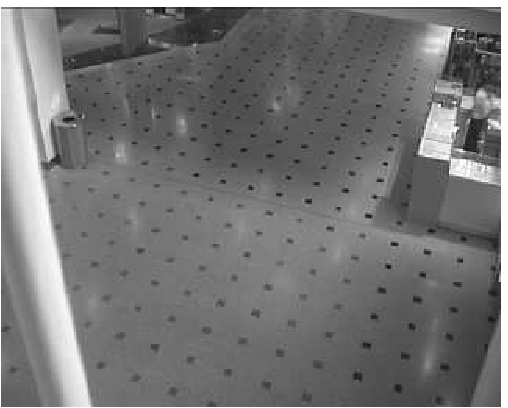
\includegraphics[scale=0.3]{figures/pcp/figure_mall_L_3.pdf} &
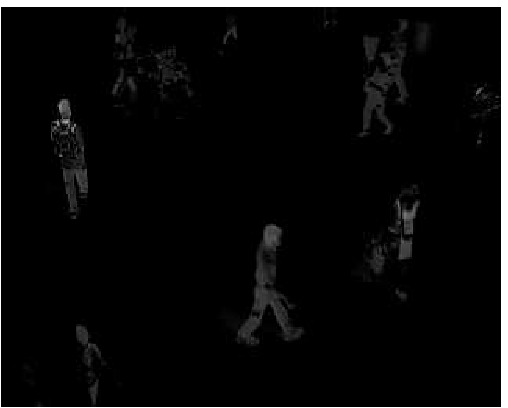
\includegraphics[scale=0.3]{figures/pcp/figure_mall_S_3.pdf} \\
\end{tabular}

\end{center}
}

\frame{\frametitle{PCP extensions}
\begin{itemize}
    \item {\makebox[4.5cm]{Square root formulation\hfill}   {\color{matbluedark}$\Rightarrow$} no parameter tuning}
    \item {\makebox[4.5cm]{Non-convex rank penalty\hfill}   {\color{matbluedark}$\Rightarrow$} better for environmental data}
    \item {\makebox[4.5cm]{Non-negativity constraint\hfill} {\color{matbluedark}$\Rightarrow$} enhanced interpretability}
    \item {\makebox[4.5cm]{Novel LOD penalty\hfill}         {\color{matbluedark}$\Rightarrow$} no need to impute}
\end{itemize}
}

% \frame{\frametitle{PCP extensions}
% \begin{itemize}
%     \item Observed value > LOD
%     \vspace{-1ex}
%         \begin{align}
%         \min_{L, S}\mathbbm{1}_{rank(L) \le r} + \lambda\|S\|_{1} + \mu\|L+S-X\|_{F}
%         \end{align}
%     \vspace{-1.5em}
%     \item Observed value < LOD \& predicted value > LOD
%     \vspace{-1ex}
%         \begin{align}
%         \min_{L, S}\mathbbm{1}_{rank(L) \le r} + \lambda\|S\|_{1} + \mu\|L+S-\delta\|_{F}
%         \end{align}
%     \vspace{-1.5em}
%     \item Observed value < LOD \& predicted value < 0
%     \vspace{-1ex}
%     \begin{align}
%     \hspace{-2em}\min_{L, S} \mathbbm{1}_{rank(L) \le r} + \lambda\|S\|_{1} + \mu\|L+S\|_{F}
%     \end{align}
%     \vspace{-1.5em}
%     \item Observed value < LOD \& predicted value [0 -- LOD]
%     \vspace{-1ex}
%     \begin{align}
%     \hspace{-8em}\min_{L, S} \mathbbm{1}_{rank(L) \le r} + \lambda\|S\|_{1}
%     \end{align}
% \end{itemize}
% }

% \frame{\frametitle{PCP extensions (plain English)}
% \begin{itemize}
%     \item No need to tune hyper-parameters
%     \item No need to impute values $<$ LOD
%     \item Strong underlying structure not assumed
%     \item Enhanced interpretability
% \end{itemize}
% \vspace{1em}
% $\Longrightarrow$
% {\color{matbluedark}\textbf{Better performance on environmental data}}}